% !TEX root = ../sethomas_thesis_main.tex

\section{Case Study: A Bistable SMA Gripper}\label{sec:smabb-gripper}
\subsection{Motivation and Background}
The core ideology behind SMA actuators has been to create miniature and compact systems that could potentially replace the current traditional solutions. In this work, the basic concept has been to discover methods by which the high energy dense nature of SMAs can be conserved when designing actuators.

This section has been motivated by the need to replace traditional pneumatic pick and place grippers that require large compressors to operate. These conventional pneumatic grippers, as they operate using compressed air and are a source of dust, are incompatible with clean-room applications. The primary motivation behind this section is to replace such a gripper and create a compact and lightweight solution that can be compatible with clean-room applications.

These pneumatic grippers are bistable grippers that fit within a small footprint with the disadvantage of requiring a wired connection to a large air compressor. Recently, SMAs have been paired with bistable elements to create actuator as shown in the work by \todocite. A simple but effective way to create a bistable element is to axially compress a beam such that they buckled. This buckled beam, which can be easily fabricated in varying dimensions, now can exist in two stable positions. The main advantage to using a bistable system is the fact that they require no additional energy to remain in these stable positions. They only require power when switching from one stable configuration to another. Thus, this behaviour can be further advantageous for designing grippers that often tend to remain in an open or closed position for extended periods of time such as drone-deliveries. As stated in previous examples, a fully compliant system can reduce the assembly complexity and weight while also preserving the life cycle if properly designed. Furthermore, a compliant bistable SMA-driven gripper can be the ideal candidate to replace the current pneumatic solution for clean-room pick and place applications.
\subsection{Working Principle and Operation}
In this design, the basic concept consists of combining antagonistic SMAs with a bistable compliant mechanism based on the proposed design methodology as described in \cref{subsec:design-methodology-antagonistic}. Using a buckled beam, a simple bistable compliant mechanism can be designed such no energy is required to remain in the open or closed position of the gripper. As previously stated, the behaviour of SMAs are difficult to model accurately and predicting the shape memory effect can be quite difficult. Similarly, multistable mechanisms with snap-through behaviours are incredibly difficult to model mathematically and therefore, system pairing both SMAs and buckled beam are used but are, often, not adequately sized. Most work such as \todocite, present such a mechanism but lack the methodology to appropriately size the SMA. The SMAs used in such systems are often oversized and present with higher cooling times degrading the time response and work density. However, in this work, using the proposed design methodology, the SMA buckled beam bistable gripper will be sized using the simplified models so as to create a gripper with reduced cooling times.

The basic principle of the presented gripper consists of using a pair of SMAs are external triggers to switch the buckled beam from one of its stable configurations to the other. In \todocite, a simple diagram of the system can be observed. Here, as mentioned, the buckled beam which is axially compressed exhibits the bistability and behaves as the compliant bistable mechanisms. The buckled beam is mounted at both ends using two supporting pivots and the snap-through is triggered by heating one of the two SMA coils. The initially straight beam, which can be fabricated as such, is buckled by bring together the support pivots. Here, one of the pivots is considered the input pivot and connected to the pair of SMA coils. The remaining pivot is considered the output and is connect to the jaws of the gripper.

The SMA coils, when heated, will contract and revert back to their original size. The input pivot is adapted to host a lever arm. As the SMA coils are allowed to contract, being attached to the lever arm, will cause the rotation of the input pivot. This rotation of the input pivot will, after a certain stroke, enable to rapid snap-through of the buckled beam switching it to its alternate stable position. Similarly, by heating the antagonistic SMA, the buckled beam can be made to switch back to its original stable position. Thus, by alternately heating either of the two SMAs, the compliant system can be made to switch back and forth between its two stable positions. As the SMA cools down, the complaint system requires no additional energy from the SMA coils to remain in the stable configurations and only requires energy when forcing the snap-through to occur.

\begin{figure}[ht!] % t for top of the page, H could be put to impose the position of the float
  \centering
  \resizebox{0.7\columnwidth}{!}{\input{images/chap7/smabb-wp-diagram_revC.pdf_tex}}
  \begin{tabular}{l@{ }l l@{ }l l@{ }l}
    {\color{mygreen} \rule[1.5pt]{10pt}{0.5mm} } & {\footnotesize 1\textsuperscript{st} Stable state} & {\color{mygreen} \rule[1.5pt]{1pt}{0.5mm} \rule[1.5pt]{1pt}{0.5mm} \rule[1.5pt]{1pt}{0.5mm}} & {\footnotesize Unstable state} &
    {\color{mygreen} \dhorline{10pt}{1.5pt}} & {\footnotesize 2\textsuperscript{nd} Stable state}\\
  \end{tabular}
  \caption{The schematic of the bistable SMA actuator composed on a buckled beam and a pair of SMA coils.}
  \label{fig:smabbwp}
\end{figure}

Compared to other bistable SMA actuators such as the work by \todocite, the real advantage of the proposed kinematic stage, using a buckled beam supported by pivots, is that gripping output is independent of the actuation input up to the point of snap-through. From the stable to unstable position of the buckled beam, the input lever makes a near full stroke while the output pivot barely rotates. As soon as the unstable position is exceeded, rapid snap-through occurs and the output pivot switches instantaneously to the other stable stage, allowing for a rapid grasping or releasing motion.
\subsection{Design of the Bistable Mechanism}
The next step, as proposed by the design methodology, consists of defining the relationship between the contract of the SMA and the kinematic stage. In this section, the analytical model of the snap-through behaviour of the proposed bistable buckled beam is established. This model can then be used to design and size the buckled beam and the SMA coils so as to create a rapidly switching gripper with the required force and stroke specifications.
\subsubsection{Analytical Model of the Buckled Beam}
A beam theory model is proposed in this section to size the bistable buckled beam mechanism for the kinematic stage. In \cref{fig:buckled-beam-schematic}, a schematic view of the buckled beam is shown. The initially flat beam buckled when compressed by a distance of $\Delta l$ by the preloading stage attached to the input pivot. The SMA is considered to apply an input torque of $M_\mathrm{in}$ at the input pivot. As the final prototype of the kinematic stage is composed completely of flexure-based mechanisms, the pivots also present with an inherent angular stiffness, $K_\mathrm{in}$ and $K_\mathrm{out}$ at the input and output pivot, respectively. The buckled beam has  flexural rigidity of $EI$ and an initial length before compression of $L$. As the flexure-based pivots are not ideal, the extremities of the beam start at a distance of $p$ from the centre of rotation of the pivots.
\begin{figure}[hbt!] % t for top of the page, H could be put to impose the position of the float
  \centering
  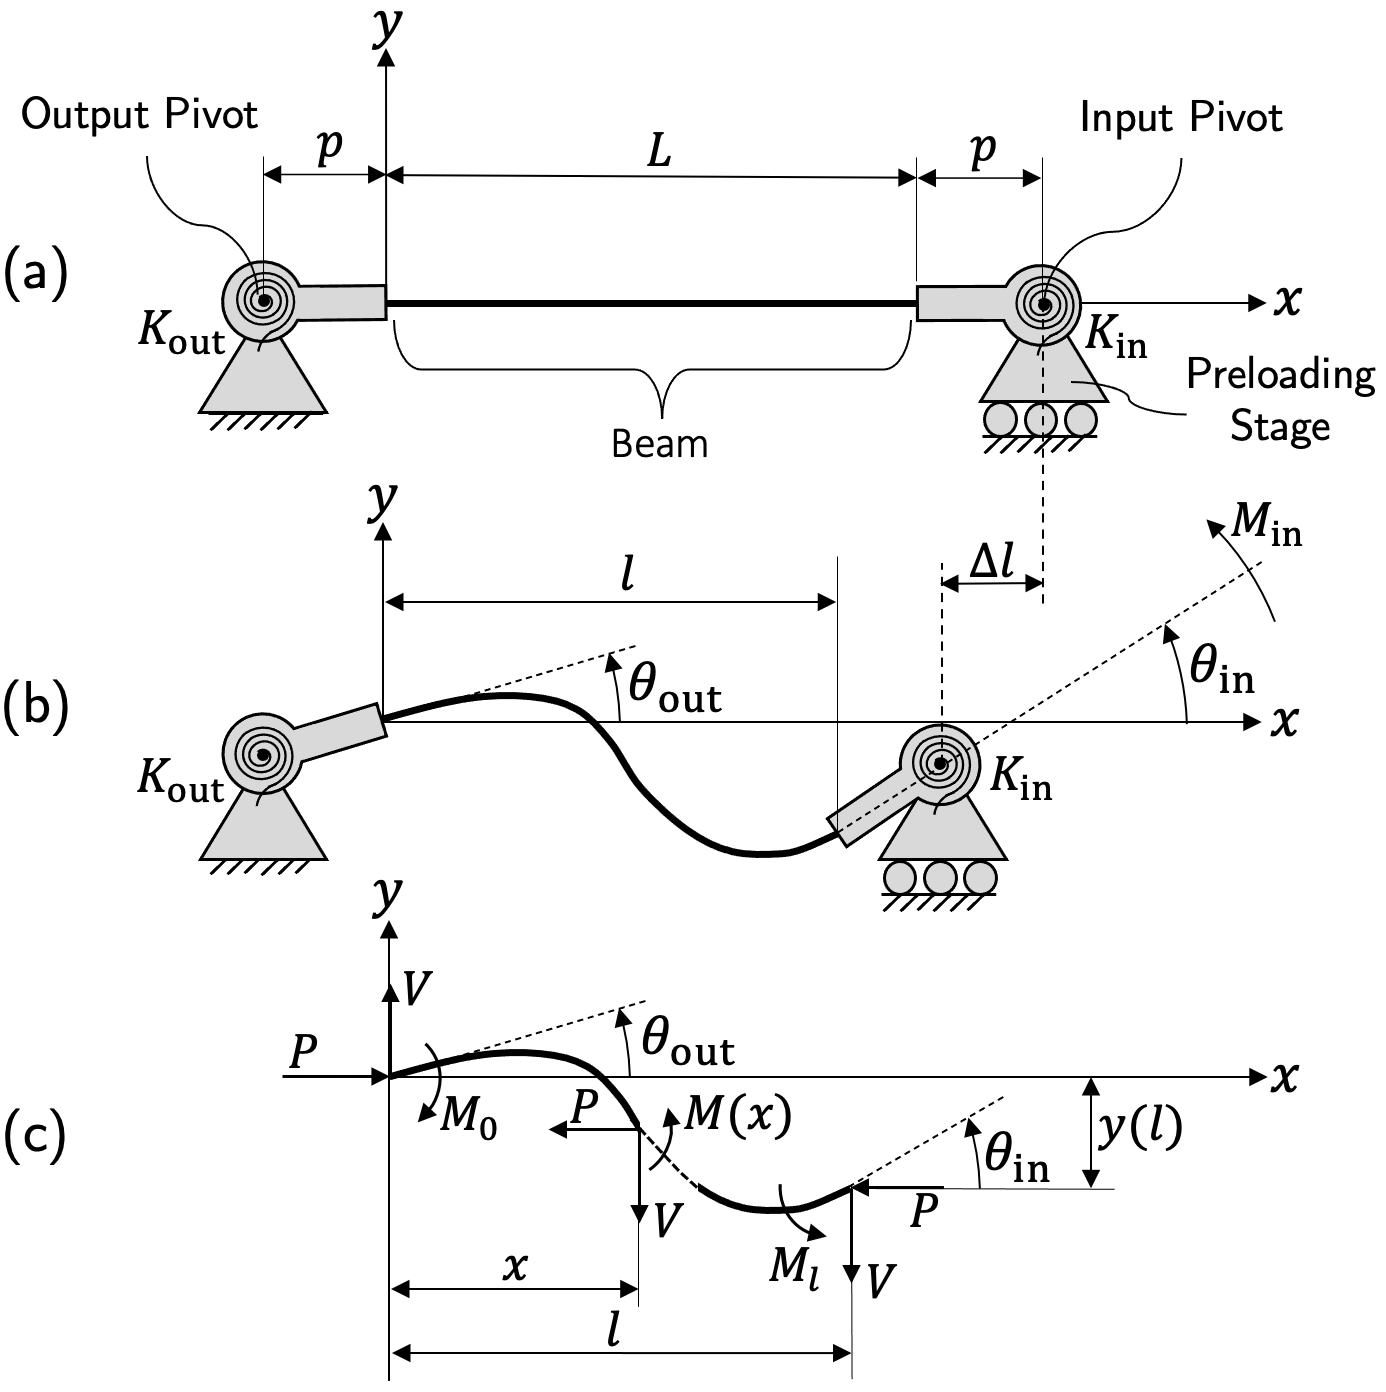
\includegraphics[width=0.7\columnwidth]{images/chap7/buckled_beam_model.png}
  \caption{(a) As-fabricated, (b) deformed and (c) free-body diagram of the buckling beam.}
  \label{fig:buckled-beam-schematic}
\end{figure}

Based on the hypothesis described in the work by \cite{tivot2021} and the Euler-Bernoulli beam theory, the beam deflection can be expressed as :
\begin{equation}\label{eq:deflection}
  y(x) = \left(A\sin{kx}+B(\cos{kx}-1)+C\frac{x}{l}\right) l {\theta }_\textrm{in}
\end{equation}
where $k=\sqrt{P/(EI)}$ and the boundary conditions are
\[y(0)=0\]
\[y'(0)\cong{\theta }_\textrm{out}\]
\[M_0\cong K_\textrm{out}\theta_\textrm{out}+Vp-Pp\theta_\textrm{out}\]
\[y(l)\cong -p(\theta_\textrm{out}+\theta_\textrm{in})\]
\[y'(l)\cong \theta_\textrm{in}\]
Furthermore, the deflection parameters are given by
\begin{equation}\label{A_norm}
A =    \frac{(1+2\overline{p})kl+{\varepsilon }_0\left(\overline{p}  \sin{kl}-\frac{\cos{kl}-1}{kl}\right)}
{kl\left( kl \cos{kl}-\sin{kl}-\left({\overline{p}}^2+\overline{p}\right){(kl)}^2\sin{kl}+{\varepsilon }_0\left(\sin{kl}+2\frac{\cos{kl}-1}{kl}\right)\right)}
\end{equation}
\begin{equation} \label{B_norm}
B = \frac{  \overline{p}(1+2\overline{p}){(kl)}^2+{\varepsilon }_0 \left(\overline{p} \left(\cos{kl}-1\right) + \frac{\sin{kl}}{kl} -1\right)}
{kl\left( kl \cos{kl}-\sin{kl}-\left({\overline{p}}^2+\overline{p}\right){(kl)}^2\sin{kl}+{\varepsilon }_0\left(\sin{kl}+2\frac{\cos{kl}-1}{kl}\right)\right)}
\end{equation}
\begin{equation} \label{C_norm}
C = \frac{  {\overline{p}}^2{(kl)}^2\sin{kl} -2\overline{p} kl\cos{kl} -\sin{kl} - {\varepsilon }_0\left(\overline{p}\sin{kl}-\frac{\cos{kl}-1}{kl}\right)}
{ kl \cos{kl}-\sin{kl}-\left({\overline{p}}^2+\overline{p}\right){(kl)}^2\sin{kl}+{\varepsilon }_0\left(\sin{kl}+2\frac{\cos{kl}-1}{kl}\right)}
\end{equation}
where $\overline{p} = p/l $ and $\varepsilon_0=K_\textrm{out}/(EI/l)$. When considering the beam’s arc length as constant, the end-shorting, $\Delta l$, can be approximated using the following expression
\begin{equation}\label{eq:delta_l}
 \Delta l\cong \frac{p}{2}({\theta }^2_\textrm{in}+\theta ^2_\textrm{out})+\int^l_0{\frac{y'(x)^2}{2}dx}=H l{\theta }^2_\textrm{in}
\end{equation}
Here, the coefficient $H$ is expressed as
\begin{multline}\label{eq:H-smabb}
 H = \frac{\left({A}^2+{B}^2\right){\left(kl\right)}^2}{4} + \frac{\left({A}^2-{B}^2\right)kl\sin{2kl} }{8} + \frac{AB kl\left(\cos{2kl}-1\right)}{4}\\
 +AC\sin{kl} + BC\left(\cos{kl}-1\right) + \frac{{C}^2}{2} +\frac{\overline{p}}{2}\left({\left( Akl+C\right)}^2+1\right)
\end{multline}

By rearranging the \cref{eq:delta_l}, the input angle is expressed as
\begin{equation}\label{eq:theta_in}
 {\theta}_\textrm{in}=\pm \sqrt{\frac{\Delta l}{l}}\sqrt{\frac{1}{H}}
\end{equation}

Finally, the input moment can be described as the following \cref{eq:M_in}
\begin{equation}
\begin{split}
 M_\textrm{in} &\cong M_l+K_\textrm{in}{\theta }_\textrm{in}+Vp-Pp{\theta}_\textrm{in}\\
 &=\frac{EI}{l}\left({\left(kl\right)}^2\left(\overline{p}\left(C-1\right)-A\sin{kl}-B\cos{kl}\right)+{\varepsilon }_l\right){\theta}_\textrm{in}
 \label{eq:M_in}
\end{split}
\end{equation}

\noindent{where ${\varepsilon }_l=K_\textrm{in}/(EI/l)$.}
\subsection{Sizing of the SMA actuator}
\subsection{Integrated Control Strategy}
\section{Conclusion}
